
%==============  N E W  ==== C H A P T E R ==============%
\chapter{Vergleich der Ergebnisse}
\label{chapter:Vergleich}

Wie in der Aufgabenstellung (siehe \ref{subsec:Ausgangslage}) erw�hnt, sollen die Suchresultate von Lucene mit denjenigen des Betriebssystems verglichen werden. Die Suche im Betriebssystem ist sehr intuitiv. Es wird der gew�nschte Suchbegriff eingegeben und nach ein paar Sekunden (oder Minuten), je nach dem ob alle Ordner indexiert waren oder nicht, erscheint das Resultat.

Die Qualit�t der Suche wird nicht anhand der Geschwindigkeit ermittelt. Anhand der im Kapitel \ref{subsec:eigesetzteHardware} aufgelisteten Hardware w�re es kein fairer Vergleich, eine SSD mit einer herk�mmlichen HDD zu vergleichen.

Um einen Vergleich zu starten, wird ein beliebiges File ausgew�hlt. Danach wird anhand nicht nur diesem File zugeordneten Kriterien gesucht. Erlaube Suchanfrage ist zum Beispiel File enth�lt \flqq beispiel\frqq, nicht jedoch filname = \flqq beispiel\frqq.

%==============  N E W  ==== S E C T I O N ==============%
\newpage
\section{Vergleich Lucene mit Windows 8.1 Pro}
\label{sec:Vergleich Lucene mit Windows 8.1 Pro}

Ausgw�hlte Datei, welche f�r gefunden werden sollte: \flqq../1. Jahr/Software Projekt 1/Dokumentation SW Projekt 2. Semester V0.1.docx\frqq

\textbf{Annahme f�r die Suche}
\begin{itemize}
\item Filename ist unbekannt
\item Autor: entweder \flqq micha\frqq\ oder \flqq reto\frqq
\item File Extension: *.doc oder *.docx
\item Im Inhalt muss vorkommen: \flqq Address.java\frqq. Dieser Teil ist der Wichtigste.
\end{itemize}

%==============  N E W  ==== S U B S E C T I O N ==============%
\subsection{Suche \#1 mit Windows 8.1 Professional}

\textbf{Suche bei Windows}\\
Bei der klassischen Suche im Windows werden die gesuchten Attribute in die Suchmaske eingegeben:
\begin{figure}[h!]
\centering
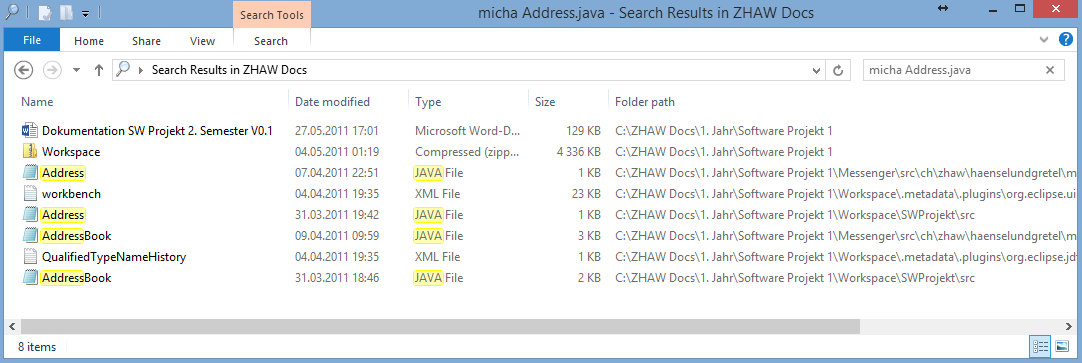
\includegraphics[width=1\textwidth]{Win8_Search1_normal.PNG} 
\caption[Gewohnte Windows Suche 1]{Gewohnte Windows Suche 1\\Quelle: eigener Screenshot}
\label{fig:Gewohnte Windows Suche 1}
\end{figure}
Die meisten Windowsbenutzer w�rden hier 2 Suchanfragen starten. Die erste mit der Suchanfrage \flqq micha Address.java\frqq, die zweite mit \flqq reto Address.java\frqq

Durch das Auseinandersetzen mit der effizienten Windows-Suche wurde klar, dass Windows von Haus aus mehr beherrscht als nur nach Stichworten zu suchen. Erweiterte Tipps f�r die Suche mit Windows gibt es von Mircosoft �ber \url{http://windows.microsoft.com/de-ch/windows7/advanced-tips-for-searching-in-windows}.

Werden die fortgeschrittenen Syntax bei der Suche eingehalten, sieht diese Anfrage folgermasse aus: \flqq authors:~="micha" OR authors:~="reto" AND Address.java\frqq. Diese Anfrage bedeutet, dass entweder \flqq micha\frqq oder \flqq reto\frqq im Feld Author vorhanden sein muss. Da \flqq Address.java\frqq nicht zugeordnet wurde, muss es irgendwo vorkommen.
\begin{figure}[h!]
\centering
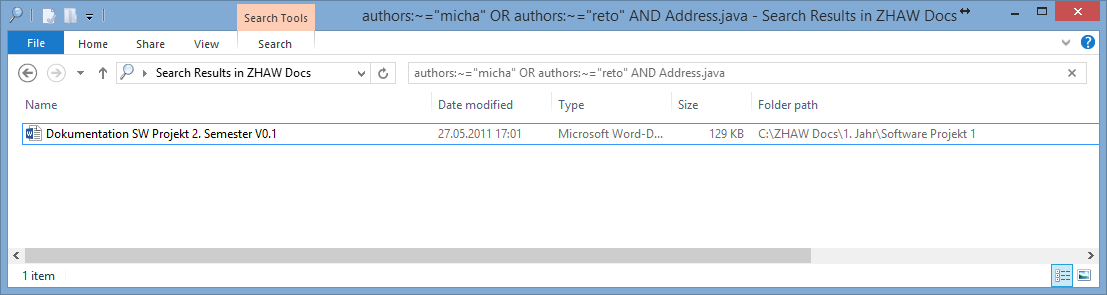
\includegraphics[width=1\textwidth]{Win8_Search1_extended.PNG} 
\caption[Erweiterte Suche 1 mit Windows]{Erweiterte Suche 1 mit Windows\\Quelle: eigener Screenshot}
\label{fig:Erweiterte Suche 1 mit Windows}
\end{figure}
  
Das Resultat mit genau einem File l�sst den Herausforderer Lucene bereits im Vorfeld keine grosse Chance.

%==============  N E W  ==== S U B S E C T I O N ==============%
\subsection{Suche \#1 mit Lucene und Luke}

Die Suche mit Luke, welche auf die von Lucene indizierte Files zugreift, dauerte im Schnitt 300-500$\mu$s.\\
Wie die Abbildung \ref{fig:Suche 1 mit Lucene} zeigt, werden hier mehrere Dateien gefunden. Die gesuchte Datei ist ebenfalls vorhanden (\#11).


\begin{figure}[h!]
\centering
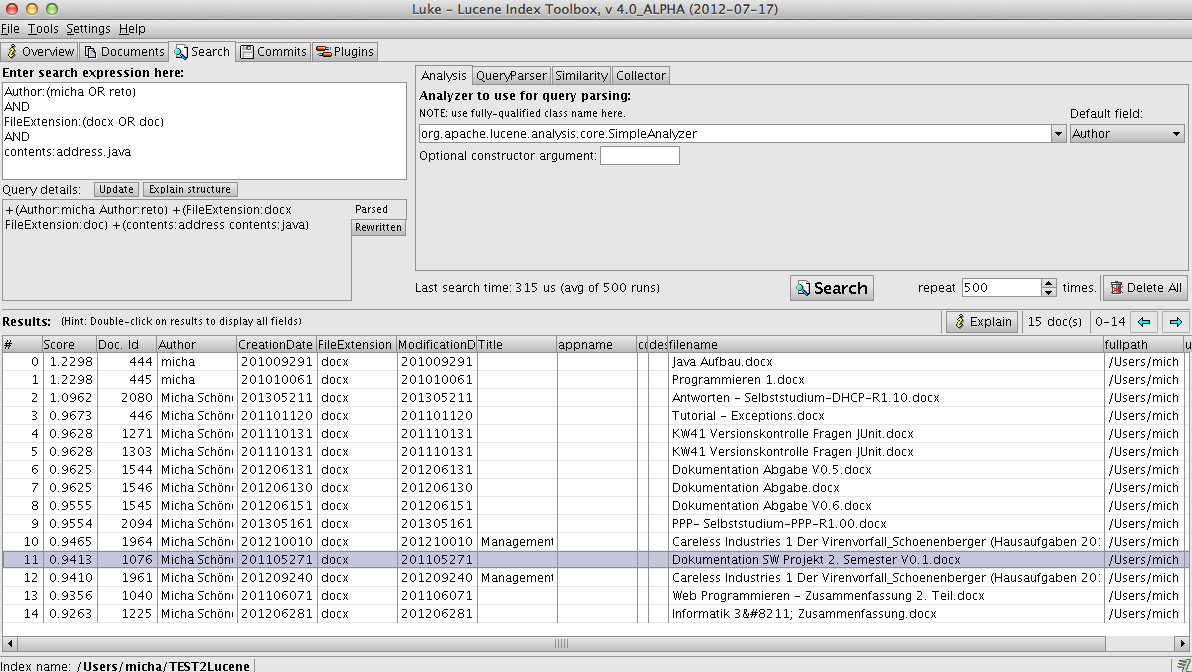
\includegraphics[width=1\textwidth]{Lucene_Search_1.PNG} 
\caption[Suche 1 mit Lucene]{Suche 1 mit Lucene\\Quelle: eigener Screenshot}
\label{fig:Suche 1 mit Lucene}
\end{figure}

%==============  N E W  ==== S U B S E C T I O N ==============%
\subsection{Fazit zur Suche \#1}

Die Windows Search Engine sowie die eigene Lucene Applikation finden beide das gew�nschte Dokument. Beim Windows ist es das einzige Dokument, welcher gelistet wird. Lucene hingegen listet das gesuchte Dokument an 11. Stelle. Ist nun Lucene schlechter deswegen?
Um auf diese Frage eine Antwort zu finden, m�ssen die anderen von Lucene ausgegebenen Dokumenten �berpr�ft werden. Es k�nnte auch sein, dass Lucene alle Dokumente auflistet, Windows jedoch nur per \grqq Zufall\grqq das richige. Was w�re, wenn das File \grqq Java Aufbau.docx\grqq, welches bei Lucene zuoberst steht, gesucht worden w�re?

Die beiden ersten Dokumente wurden untersucht. Das Fazit hierbei ist, dass aller Merkmale perfekt getroffen haben bei Lucene, ausser dem contents:address.java. \flqq address.java\frqq\ wurde in beiden Dokumenten nicht gefunden. Wo liegt der Fehler?


Wird die identische Suche mit Luke nochmals durchgef�hrt, jedoch anstelle des Standard-Analyzer der German- oder English-Analyzer eingesetzt, findet Lucene genau eine einzige Datei (siehe Abbildung \ref{fig:Suche 1 mit Lucene English Analyzer}). Es ist genau die Datei, die gesucht wurde.

\begin{figure}[h!]
\centering
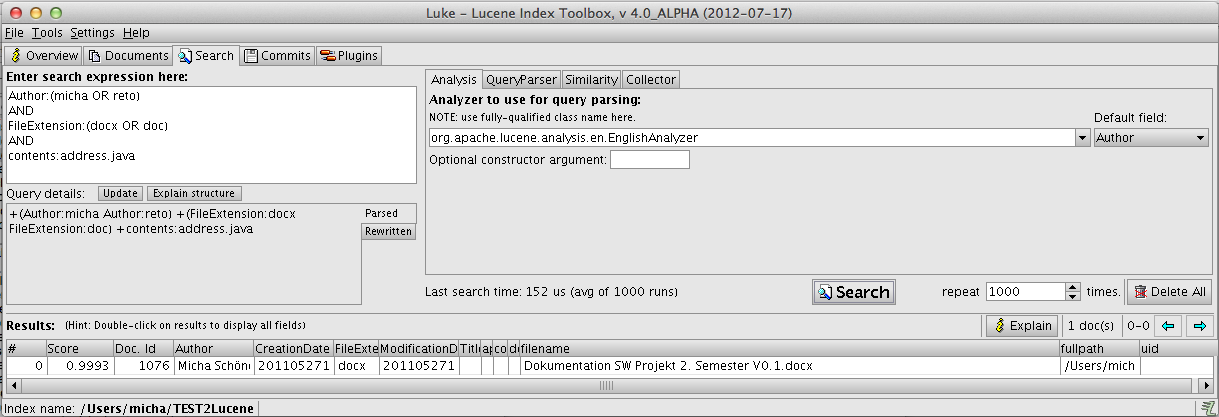
\includegraphics[width=1\textwidth]{Lucene_Search_1_english.PNG} 
\caption[Suche 1 mit Lucene mit English-Analyzer]{Suche 1 mit Lucene mit English-Analyzer\\Quelle: eigener Screenshot}
\label{fig:Suche 1 mit Lucene English Analyzer}
\end{figure}


\textcolor{red}{HIER ERKL�REN WAS UNTERSCHIED VON ANALYZERN IST}

%==============  N E W  ==== S E C T I O N ==============%
\section{Vergleich 2 Lucene mit Windows 8.1 Pro}
\label{sec:Vergleich 2 Lucene mit Windows 8.1 Pro}
























